\subsection{Pre-processing}
Before extracting the planes, we preprocessed the range data to eliminate the background since the only things we are interested are the cabinet and the book, which are in the foreground. After having observed the range data, we decided to eliminate all pixels with the range $Z > 1400$, which removed the background. Additionally we transformed the range data in X-Y space to a pointcloud which made it easier to work with and visualize (see Figure \ref{fig:foundation}).

For registering views we decided to use frame number 17 as our foundation frame (see Figure \ref{fig:foundation}) which we used for computing the rotation and translation between that frame and all the others.

\begin{figure}[H]
	\centering
	\begin{subfigure}[b]{0.45\textwidth}
		\centering
		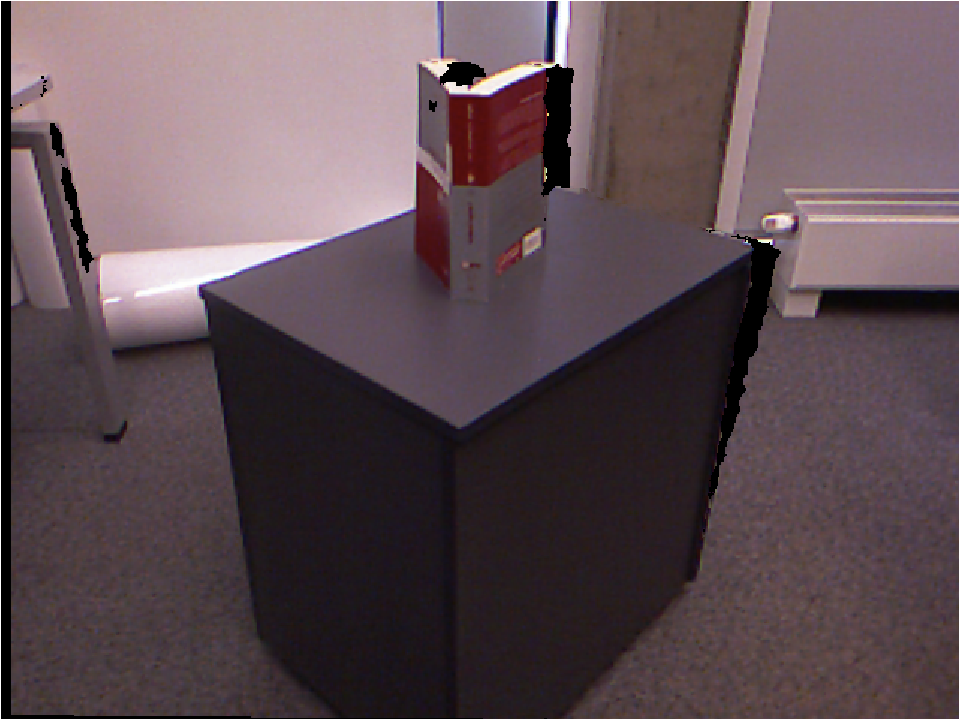
\includegraphics[width=\textwidth]{Images/1-Image(1).png}
		\caption{}
	\end{subfigure}%
	\hspace{1cm}
	\begin{subfigure}[b]{0.45\textwidth}
		\centering
		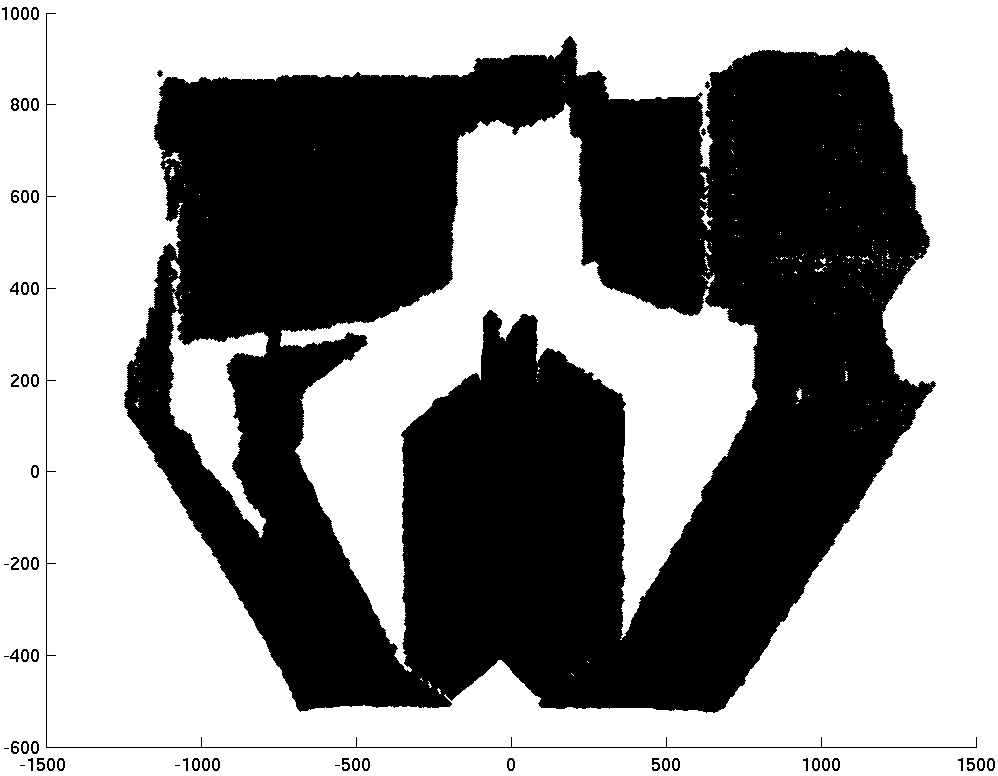
\includegraphics[width=\textwidth]{Images/2-Range(1).png}
		\caption{}
	\end{subfigure}
	\caption{The image (a) and X-Y range data converted to a point cloud (b) for our foundation frame.}
	\label{fig:foundation}
\end{figure}